\documentclass[12pt]{article}
\usepackage[utf8]{inputenc}
\usepackage[T1]{fontenc}
\usepackage[norsk]{babel}
\usepackage{floatpag}				% Different pagestyles
\usepackage{amsmath}
\usepackage{array}	
\usepackage{booktabs}
\usepackage{amssymb}
\usepackage{graphicx}
\usepackage{epstopdf}
\usepackage{tabularx}
\usepackage{float}
\usepackage{caption}
\usepackage{subcaption}
\usepackage{parskip}
\usepackage{multirow}
\usepackage{listings}


\begin{document}
\title{Oblig3}
\author{Magnus Isaksen}
\maketitle

\section*{0.3}

\subsection*{a)}

For å finne antall ledige tilstander bruker vi 

$\Omega(n) = \frac{N!}{n!(N-n)!} $

\subsection*{b)}

Entropi er gitt ved 

$S = k\ln \Omega$

Hvor $\Omega$ er fra forrige deloppgave. Dette gir

$S = k\ln (\frac{N!}{n!(N-n)!})$

Sterlings tilnærming gir oss 

$S = k(\ln(N!) -\ln(n!) -\ln(N-n)!)$

\subsection*{c)}
Hvis da N>>n 

Kan vi tilnærme 

$ S = k((N\ln(N) -N) - (n\ln(n) -n) - ((N-n)\ln(N-n) -(N-n)))$



\subsection*{d)}

Temperaturen finner vi ved 

$\frac{1}{T} = \frac{dS}{dU}$

Hvor U er den totale energien.

$U = \Delta \epsilon n$

Noe som gir oss ledige plasser n. 

$n = \frac{U}{\Delta \epsilon}$

Vi bruke

$\frac{dS}{dU} =\frac{dS}{dn}\frac{dn}{dU} $

Da får vi 

$\frac{dS}{dn} = k ((-\ln n + n\frac{1}{n}) -(-\ln (N-n) +(N-n)\frac{1}{N-n}(-1))$

$\frac{dS}{dn} = k(-\ln n -1 + \ln (N-n) +1)$

$ \frac{dS}{dn}= k(\ln (N-n) -\ln n)$

$ \frac{dS}{dn}= k(\ln N(1 -\frac{n}{N}) -\ln n) = k(\ln N -\ln n) = k \ln\frac{N}{n}$


Så ser vi på $\frac{dn}{dU}$

$\frac{dn}{dU} = \frac{d(\frac{U}{\Delta \epsilon}}{dU} = \frac{1}{\Delta \epsilon}$

Da får vi at 

$\frac{1}{T} = \frac{k\ln (\frac{N}{n}}{\Delta \epsilon}$

og tilslutt har vi temperaturen

$T = \frac{\Delta \epsilon}{k\ln (\frac{N}{n}}$

\subsection*{e)}

Skal nå se på hvor mange ledige plasser det er som funksjon av T.

$T = \frac{\Delta \epsilon}{k\ln (\frac{N}{n}}$

$k(\ln N -\ln n) = \frac{\Delta \epsilon}{T}$	

$\ln n =\ln N - \frac{\Delta \epsilon}{kT}$	

$ n = e^{\ln N -\frac{\Delta \epsilon}{kT}}$

$ n = Ne^{-\frac{\Delta \epsilon}{kT}}$

Her ser vi at n er avhengig av hvordan T oppfører seg så n er en "fluctuating value".

\subsection*{f)}

Når temperaturen går mot null går også uttrykket mot null, så da er det ingen ledige plasser. 

\subsection*{g)}

Plotter antall ledige plassr i python og får Figur\ref{temp}

\begin{lstlisting}

from pylab import *
from numpy import *
import matplotlib.pyplot as mp
N = 10**23
deps = 1.0 #ev
kb = 8.617e-5 #eV/K Boltzmann
T = linspace(40,1000,100000)
rt = len(T)
n = zeros(rt)

for i in range(rt):
    n[i] = N*exp(-deps/(kb*T[i]))
#plotting vacancies 
mp.plot(T,n)
mp.xlabel('Temperature')
mp.ylabel('Vacancies')

#finding heat capasity
c = (deps**2*N/(kb*T**2))*exp(-deps/(kb*T))

mp.figure()
mp.plot(T,c)
mp.xlabel('Temperature ')
mp.ylabel('Heat capacity')
mp.show()

\end{lstlisting}


\begin{figure}[hb!]
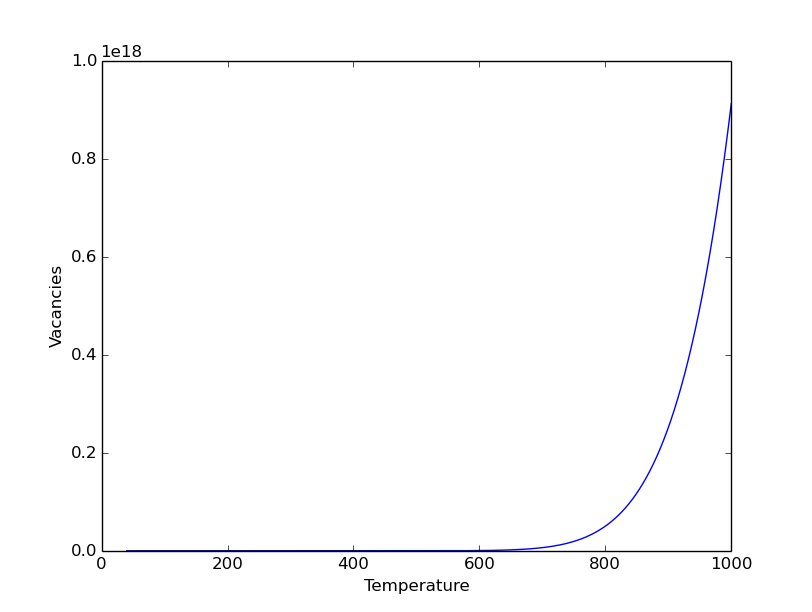
\includegraphics[width = \textwidth]{vacancies}
\caption{Ledige plasser som funksjon av temperatur}
\label{temp}
\end{figure}

\subsection*{h)}

Varmekapasitet finner vi ved 

$c = \frac{dU}{dT}$

hvor $U = \Delta \epsilon n = \Delta \epsilon Ne^{-\frac{\Delta \epsilon}{kT}}$

Deriverer vi får vi 

$c = \Delta \epsilon N \frac{\Delta \epsilon}{kT^2}e^{-\frac{\Delta \epsilon}{kT}} = \frac{\Delta \epsilon^2N}{kT^2}e^{-\frac{\Delta \epsilon}{kT}}$ 

Plotter vi denne får vi Figur \ref{heat} og vi ser at den øker med temperaturen på samme måte som antall ledige plasser gjør. Så med høyere temperatur er varmekapasiteten høyere. 

\begin{figure}[hb!]
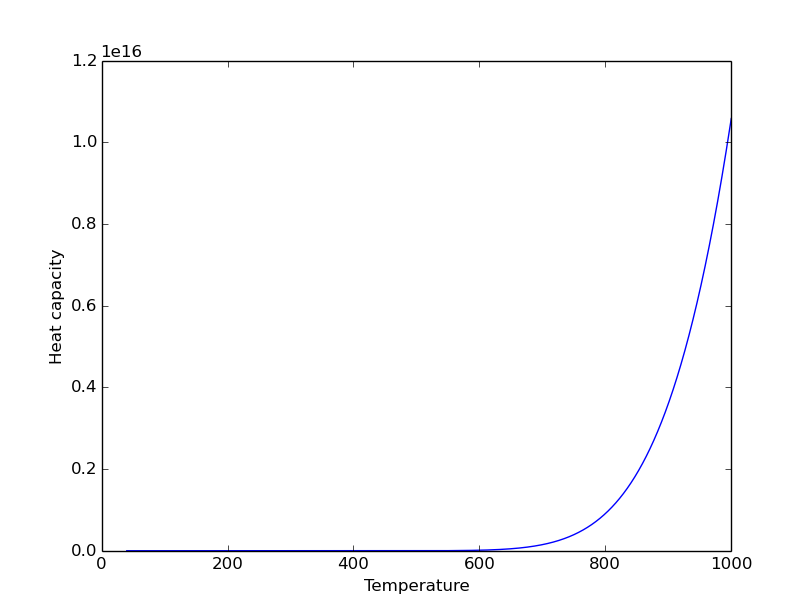
\includegraphics[width = \textwidth]{heatcap}
\caption{Varmekapasitet dom funksjon av temperatur}
\label{heat}
\end{figure}

\section*{0.4}

\subsection*{a)}

Multiplisiteten finner vi med 

$\Omega(N_R) = \frac{N!}{N_R!(N-N_R)!}$

Hvor N er det totale antall polymer og $N_R$ er de som peker mot høyre. 

\subsection*{b)}

Lengden til kjeden er antall som peker mot høyre minus de som peker mot venstre. 

$L = \Delta l (N_R -(N-N_R)) = \Delta l (2N_R -N)$

\subsection*{c)}

Finner først at $N_R = \frac{L}{2\Delta l}$

Setter dette inn i formelen for entropi

$S = k \ln \Omega$

$S = k\ln (\frac{N!}{N_R!(N-N_R)!})$

$S = k \ln (\frac{N!}{(\frac{L}{2\Delta l} +\frac{N}{2})!(\frac{N}{2}-\frac{L}{2\Delta l}})$

\subsection*{d)}

Vi vet at $dE = TdS -PdV$

Og her er F=-P og dV lik dL da vi ser på en dimensjon. 

Slik at med omrokkering.

$TdS = dE -FdL$

\subsection*{e)}

$FdL = dE -TdS$

$F = \frac{dE}{dL} -T\frac{dS}{dL}$

Vi vet at den totale energien er bevart så $\frac{dE}{dL} = 0$

Dermed får vi 

$F = -T\frac{dS}{dL}$

Tar så å ser på 

$\frac{dS}{dL} = \frac{dS}{dN_R}\frac{dN_R}{dL}$

$\frac{dS}{dN_R} = \frac{d}{dN_R} k(\frac{N!}{N_R!(N-N_R)!})$

$\frac{dS}{dN_R} = \frac{d}{dN_R} k (N\ln N +N -N_R\ln N_R -N_R -(N-N_R)\ln (N-N_R) -(N-N_R))$

$\frac{dS}{dN_R} = k(\ln (N-N_R) +(N+N_R)(\frac{1}{(N+N_R)}-\ln N_R -1)$

$\frac{dS}{dN_R} = k(\ln(N-N_R) -\ln N_R)$

Deretter finner vi $\frac{dN_R}{dL}$

$N_R = \frac{L}{2\Delta l} + \frac{N}{2}$

$\frac{dN_R}{dL} = \frac{1}{2\Delta l}$

dette gir

$\frac{dS}{dL} = \frac{k (\ln (N-N_R) -\ln N_R)}{2\Delta l}$

Setter vi inn dette får vi

$ F = -\frac{Tk}{2\Delta l}(\ln(N-N_R) -\ln N_R$

$ F = -\frac{Tk}{2\Delta l}(\ln(\frac{N}{2} -\frac{L}{2\Delta l}) -\ln (\frac{L}{2\Delta l} + \frac{N}{2})$

$F = -\frac{Tk}{2\Delta l}(\ln (N\Delta l +L) - \ln (N\Delta l- L)$

\subsection*{f)}


Hooks lov gir oss $F = -kx$ hvor x er lengden.

$F = -\frac{Tk}{2\Delta l}(\ln (N\Delta l +L) - \ln (N\Delta l- L)$

Når $L<<N\Delta l$

$F = -\frac{Tk}{2\Delta l}(\ln (N\Delta l(1 +L\frac{L}{N\Delta L}) - \ln (N\Delta l(1- \frac{L}{N\Delta L}) = -\frac{Tk}{2\Delta l}2\frac{L}{N\Delta L} =  -\frac{Tk}{2\Delta l^2}L$

Som da oppfyller Hooks lov ved at vi har en konstant foran lengden L dersom temperaturen holder seg konstant. 

\subsection*{g)}

Dersom temperaturen øker vil krafta trekkes inn og dersom T er mindre vil den strekkes letter. Nei det gir ikke helt mening for meg, jeg ville tro at det burde være motsatt. 

\subsection*{h)}
Jeg vil forvente at temperaturen vil øke da vil tilfører et arbeid, og det vil være friksjon til å varme den opp. 



\end{document}